\section{Appendix}

\subsection{Prompts for Query Decomposition}\label{sec:prompts}
The NeuCLIR dataset contains complex user requests and associated nuggets with annotated documents. We thus generate our own query decomposition using LLM calls. We decompose each NeuCLIR user request into \(k=16\) sub-queries using prompts \ref{fig:problem-definition-prompt} and \ref{fig:specialized-information-prompt}.

\begin{figure*}[!ht]
  \centering
    \begin{subfigure}{\linewidth}
	\begin{tcolorbox}[colback=gray!5!white, colframe=black!75!black, boxrule=0.5pt, arc=3pt, left=6pt, right=6pt, top=4pt, bottom=4pt]
	
	\textbf{Prompt for generating Problem Definition Search Queries}

	You are an assistant that receives a complex user request and must generate search queries whose answers:
	(1) define the user's request, and 
	(2) define all key entities mentioned in the request.
	
	\begin{enumerate}
		\item Consider any current events, recent developments, or specific details mentioned in the context to enhance the queries (if context is provided).
		\item Write \textbf{up to \texttt{<<no\_queries>>}} objective Google search queries related to the request.\\
		      The queries should be general and high-level (e.g., encyclopedic or definitional in nature).\\
		      Avoid narrow or overly specific phrasings. Queries should be phrased as something someone would realistically search for.
		\item Assume the current date is \texttt{<<current\_date>>} if required by the request.
		\item Return the queries as a JSON list of strings in the format: \\
		      \texttt{["query 1", "query 2", "query 3"]}.\\
		      The response must contain \textbf{only} this list.
	\end{enumerate}
    \end{tcolorbox}
    \end{subfigure}
  \caption{Prompt for Generating Problem Definition Queries}
  \label{fig:problem-definition-prompt}
\end{figure*}

\begin{figure*}[!ht]
  \centering
    \begin{subfigure}{\linewidth}
    \begin{tcolorbox}[colback=gray!5!white, colframe=black!75!black, boxrule=0.5pt, arc=3pt, left=6pt, right=6pt, top=4pt, bottom=4pt]
    
    \textbf{Prompt for Generating Specialized Information Search Queries}

    You are a seasoned research assistant tasked with generating search queries that ask highly specialized and detailed information about a user request. You have access to a context formed of multiple supporting documents.

    \begin{enumerate}
        \item Use the context (if provided) to identify aspects of the request that would benefit from more specific, in-depth, or expert-level information.\\
              Consider any current events, real-time developments, or precise facts that can be used to craft better questions.
        \item Write \textbf{up to \texttt{<<no\_queries>>}} objective Google search queries related to the request.\\
              These queries should be highly specific and targeted—something a person wouldn't know from general knowledge.\\
              Each query should reflect a concrete sub-aspect or follow-up inquiry about the original request.
        \item Assume the current date is \texttt{<<current\_date>>} if required by the request.
        \item Return the queries as a JSON list of strings in the format: \\
              \texttt{["query 1", "query 2", "query 3"]}.\\
              The response must contain \textbf{only} this list.
    \end{enumerate}
    \end{tcolorbox}
    \end{subfigure}
  \caption{Prompt for Generating Specialized Information Queries}
  \label{fig:specialized-information-prompt}
\end{figure*}

\subsection{Gaussian Distributions}\label{sec:gaussian}

\header{Gaussian estimates} The finding in Figure \ref{fig:slope_neuclir} serves as an explanation to the Gaussian policies performing considerably poorly compared to the Bernoulli ones, as seen Table \ref{tab:Gaussian_alpha_ndcg}. This suggests that Gaussian distributions may not be suited to capturing relevance when the ranking signal is noisy. 

\begin{algorithm}[ht]
\caption{Thompson Sampling in Continuous Space}\label{tab:thompson_continuous_space}
\SetKwInOut{Input}{Input}
\SetKwInOut{Output}{Output}
\Input{Sub-queries $\mathcal{S} = \{s_1, \dots, s_K\}$}
\Input{Budget $b$}
\BlankLine

\For{$i = 1,\dots,K$}{
    Define Gaussian priors $\mathcal{N}(\mu_0, \sigma_0^2)$ where $\mu_0 \gets 0$ and $\sigma_0^2 \gets 1$ \\
}

\For{$t = 1,\dots,b$}{
    \For{$i = 1,\dots,K$}{
        Sample from posterior $\theta_i \sim \mathcal{N}(\mu_i,\sigma^2_i)$
    }
    Select arm (sub-query): $a_t \gets \arg\max_{i} \theta_i$ \\
    
    Pick next document $d_{a_t, n} \in \mathcal{D}_{a_t}$ where \\
    \hspace{1em} \(n = \min \{ j \in \{1,\ldots,N\} \mid (a_t, j) \notin \mathcal{O} \}\)
    
    Observe the likelihood: $r(a_t, n)$

    Update posterior: \\
       \hspace{1em} $\sigma_{a_t}^2 = \sqrt{(\frac{1}{\sigma_0^2} + n)^{-1}}$ \\
       \hspace{1em} $\mu_{a_t} = \sigma_{a_t}^2 \cdot \sum_{r \in {S_{a_t}}} r$
}
\end{algorithm}

\subsection{Report Generation Example}\label{sec:app_report_gen_example}
In this section, we show an example of a report generated and evaluated using Auto-ARGUE.

\header{Query} What characterizes Ernest Hemingway’s writing style, and what is the “iceberg theory”?

\header{Generated report} Ernest Hemingway was a renowned American writer known for a distinctive style built on simplicity, clarity, and concrete detail \([5]\).
He is often associated with the “iceberg theory,” the idea that most meaning lies beneath the surface while only a small portion is stated explicitly \([3],[5]\).
Hemingway’s years as a journalist shaped this approach: he learned to write concise, unadorned prose that focuses on essentials \([2]\).
He also insisted on authenticity—“never write about what you do not know”—and favored describing observable actions while letting readers infer the emotions behind them \([1]\).
This restrained, lucid style has been widely emulated and is a major reason he is regarded as one of the most influential writers of the twentieth century \([4]\).


\subsection{Complete results on NeuCLIR and ResearchyQuestions}

Figures~\ref{fig:neuclir_precision_all}–\ref{fig:researchy_recall_all} report precision and recall across budgets for all baselines and bandit policies we introduce in Table \ref{tab:reward_functions}. Figure ~\ref{fig:researchy_correlated} compared serial and hierarchy-aware document selection. 

\begin{figure*}[t]
    \centering
    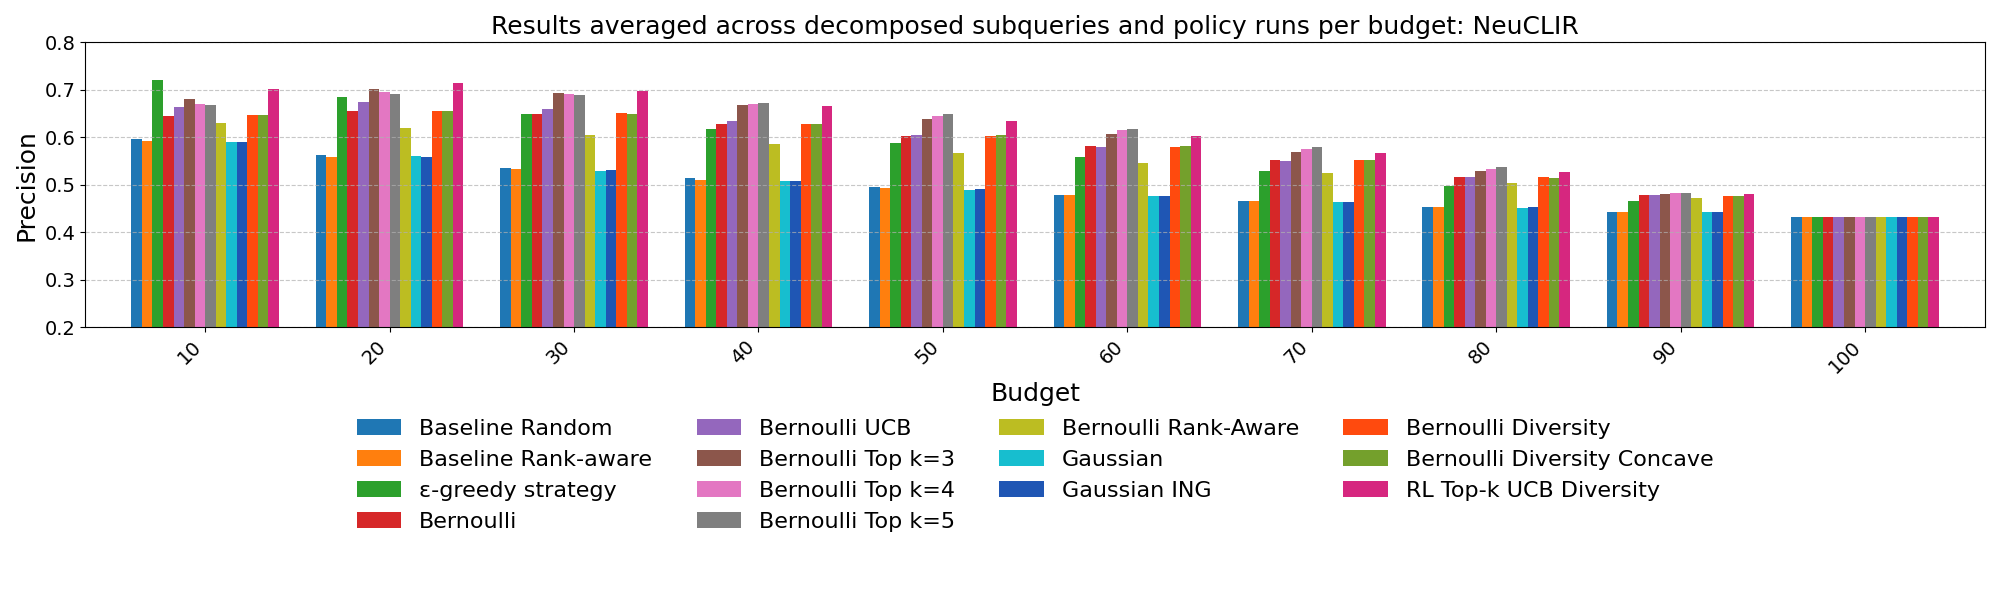
\includegraphics[width=\linewidth]{images/NeuCLIR/precision_all_small_axis.png}
    \caption{Precision applying baselines and reward policies for query selection for different budgets over observed documents. The budget is calculated as a percentage over the total amount of available documents. Modelling the queries using Bernoulli distribution considering the top ranked k documents performs the best across budgets, with all policies reaching the same performance as the budget covers the whole space of actions.}
    \label{fig:neuclir_precision_all}
\end{figure*}

\begin{figure*}[t]
    \centering
    
\includegraphics[width=\linewidth]{images/Researchy/precision_all_small_axis.png}
    \caption{Precision applying baselines and reward policies for query selection for different budgets over observed documents in ResearchyQuestions. The budget is calculated as a percentage over the total amount of available documents. Modeling the queries using Bernoulli distribution considering the top ranked k documents performs the best across budgets, with all policies reaching the same performance as the budget covers the whole space of actions.}
    \label{fig:researchy_eval_all}
\end{figure*}


\begin{figure*}[t]
    \centering
    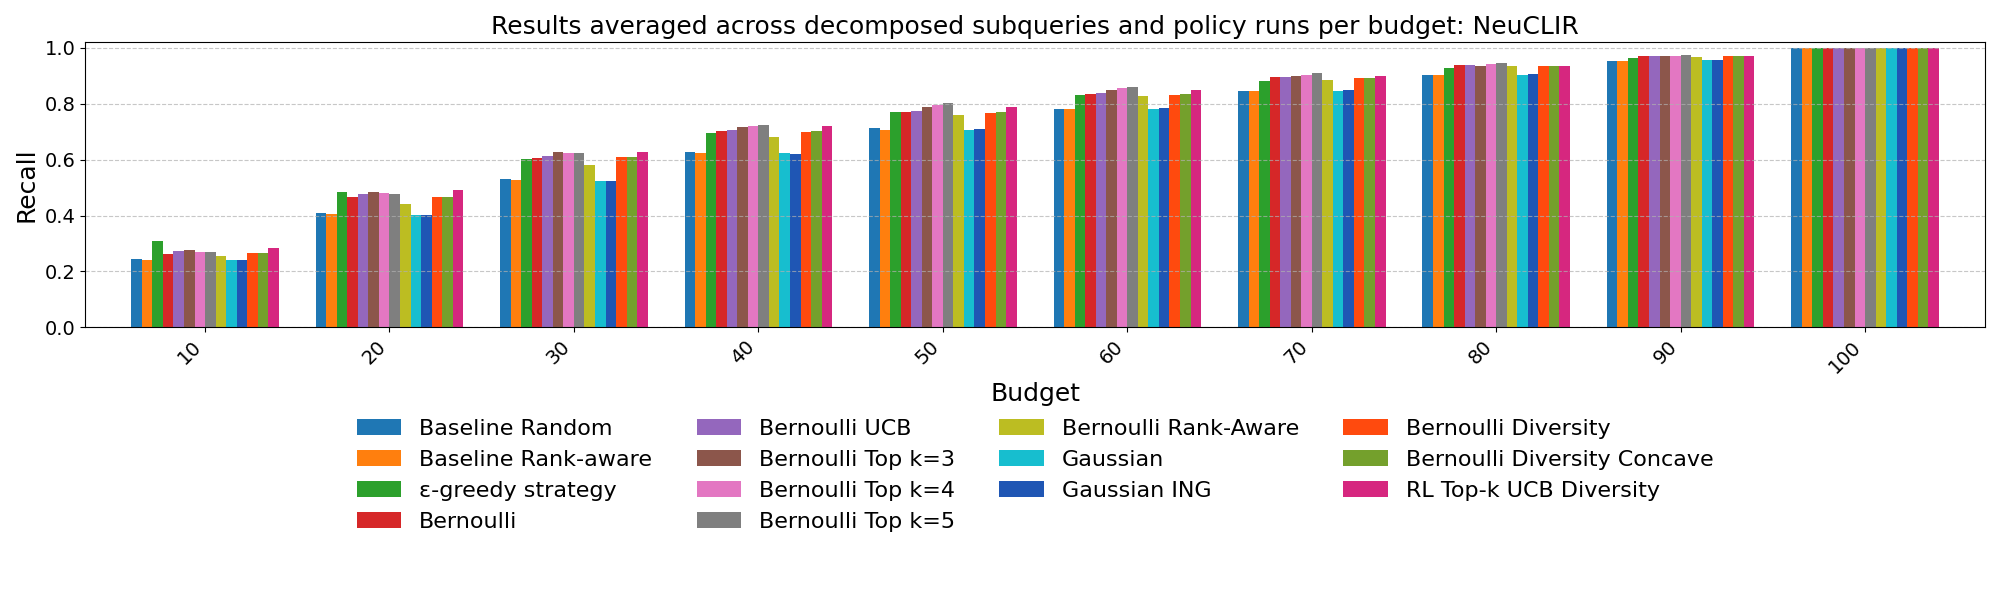
\includegraphics[width=\linewidth]{images/NeuCLIR/recall_all_big_axis.png}
    \caption{Recall applying baselines and reward policies for query selection for different budgets over observed documents. The budget is calculated as a percentage over the total amount of available documents. Modelling the queries using Bernoulli distribution considering the top ranked k documents performs the best across budgets, with all policies reaching the same performance as the budget covers the whole space of actions.}
    \label{fig:neuclir_recall_all}
\end{figure*}

\begin{figure*}[t]
    \centering
    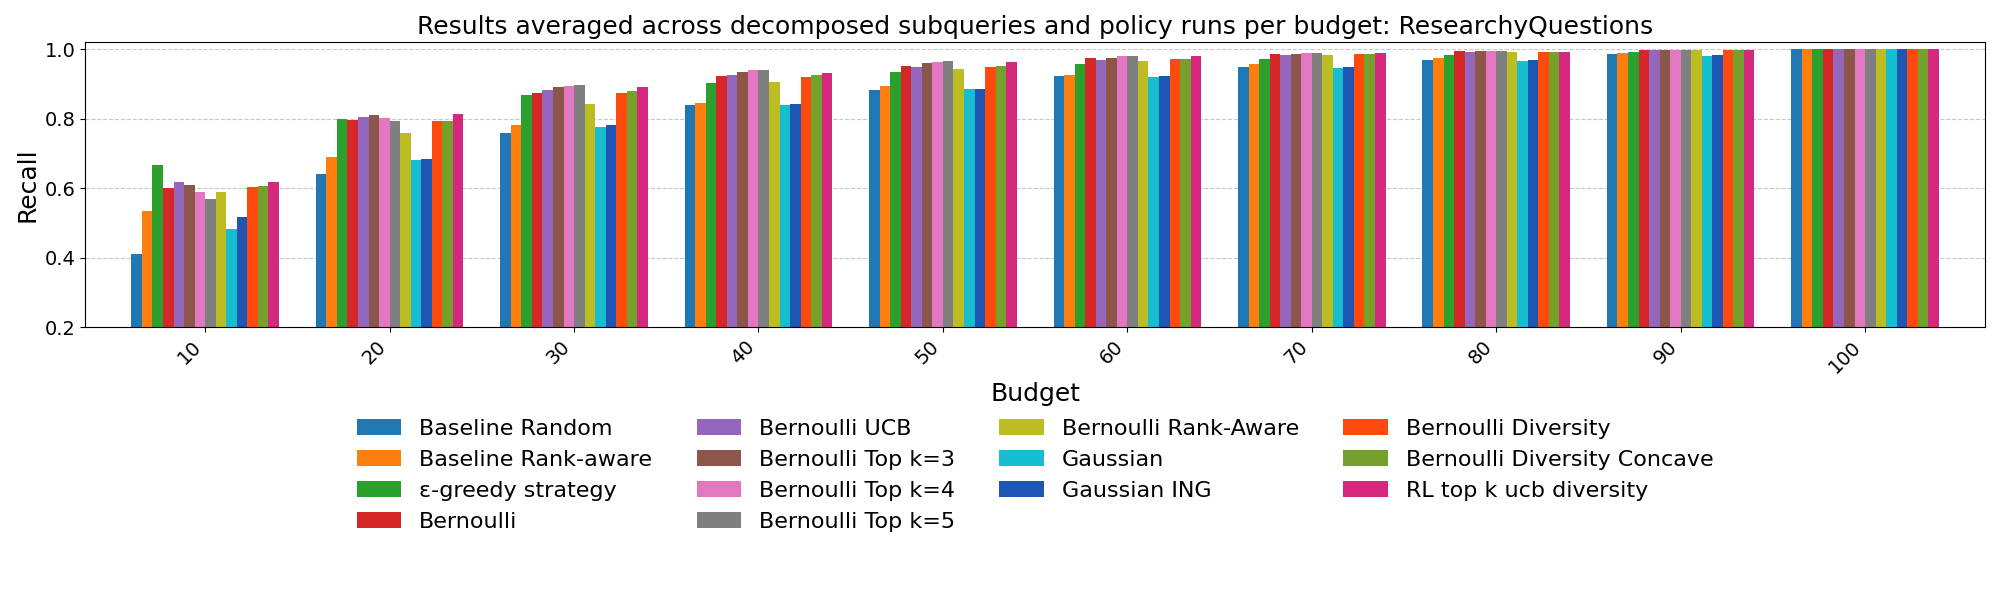
\includegraphics[width=\linewidth]{images/Researchy/recall_all_small_axis.png}
    \caption{Recall applying baselines and reward policies for query selection for different budgets over observed documents in ResearchyQuestions. The budget is calculated as a percentage over the total amount of available documents. Modeling the queries using Bernoulli distribution considering the top ranked k documents performs the best across budgets, with all policies reaching the same performance as the budget covers the whole space of actions.}
    \label{fig:researchy_recall_all}
\end{figure*}

\begin{figure*}[t]
    \centering
    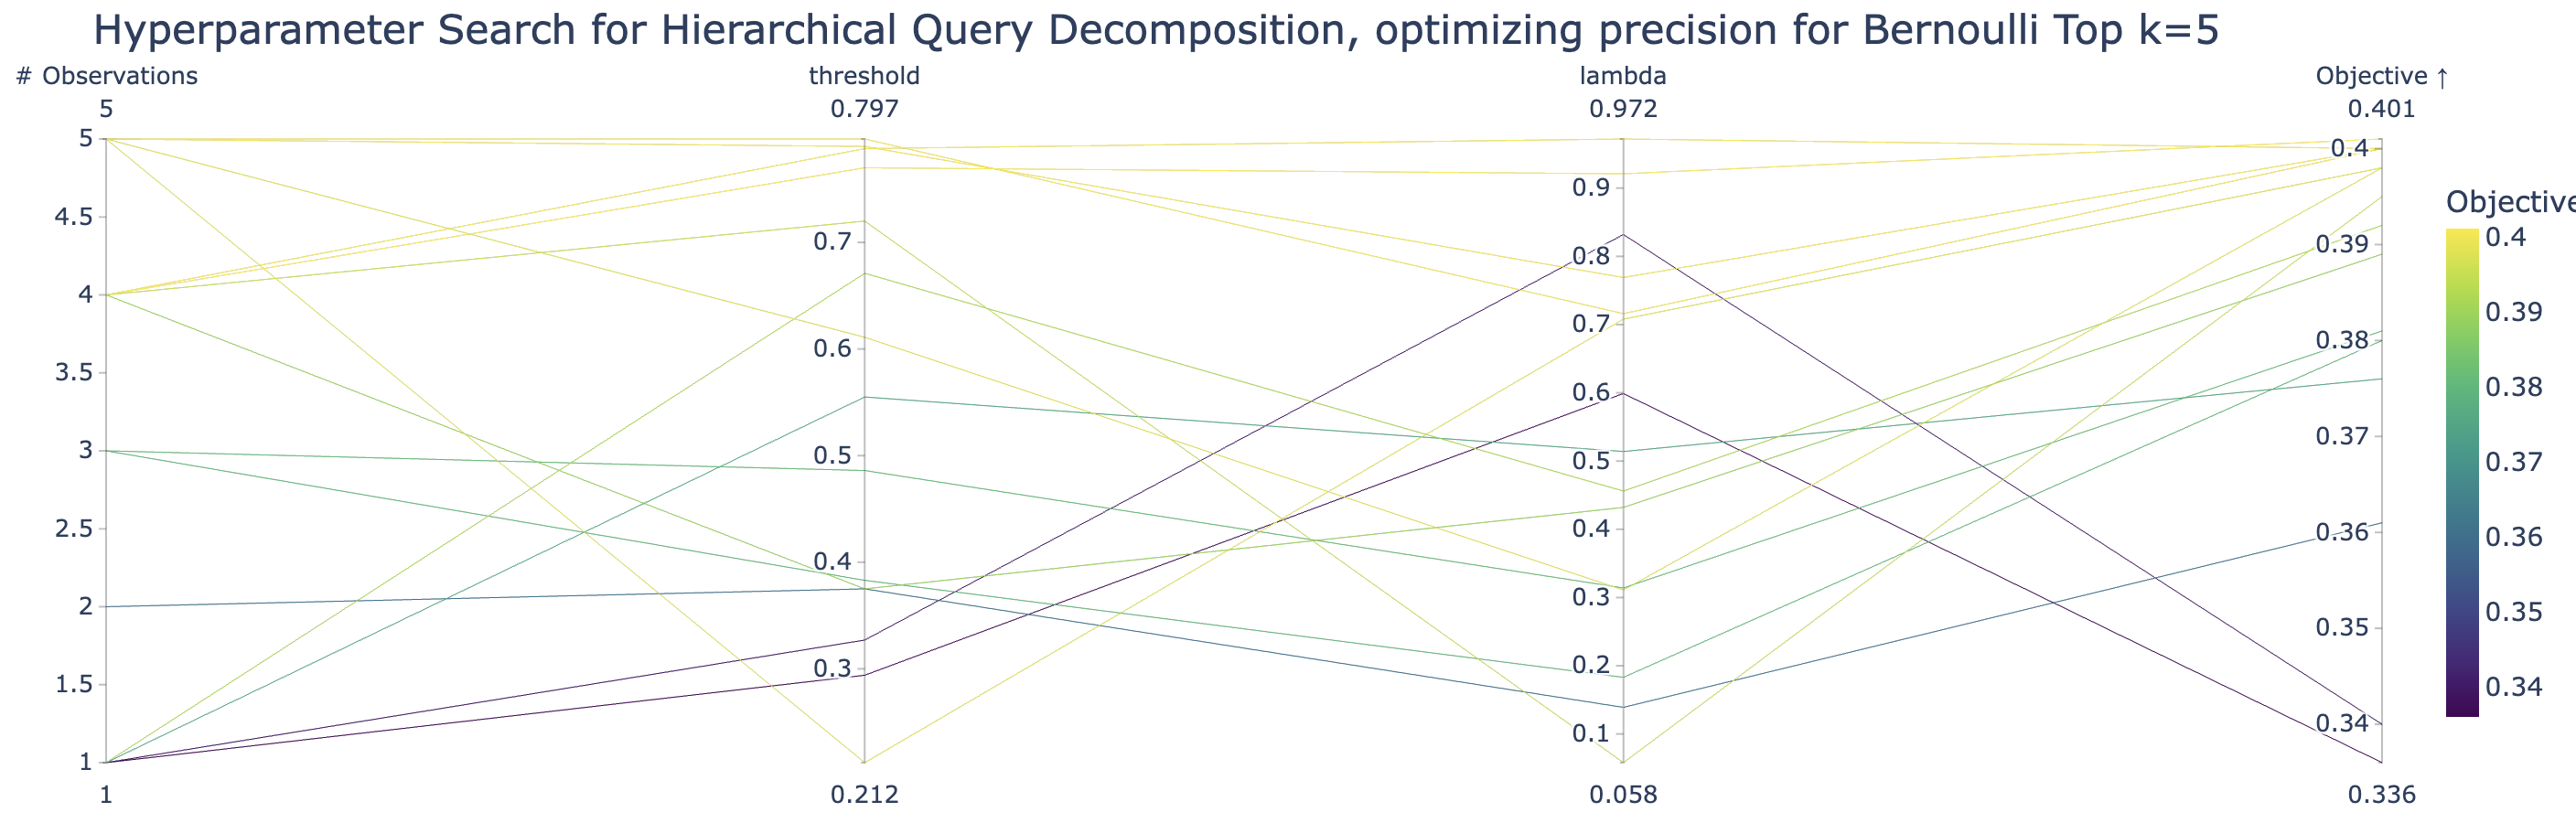
\includegraphics[width=\linewidth]{images/Researchy/bayesian_lookup.png}
    \caption{Visualization of hyperparameter search space with Bayesian optimization on the precision objective of the RL top k = 5 approach on the Researchy dataset. Each line corresponds to a trial with specific values of the three hyperparameters, colored according to the achieved objective.}
    \label{fig:bayesian_lookup}
\end{figure*}


\begin{figure*}[t]
    \centering
    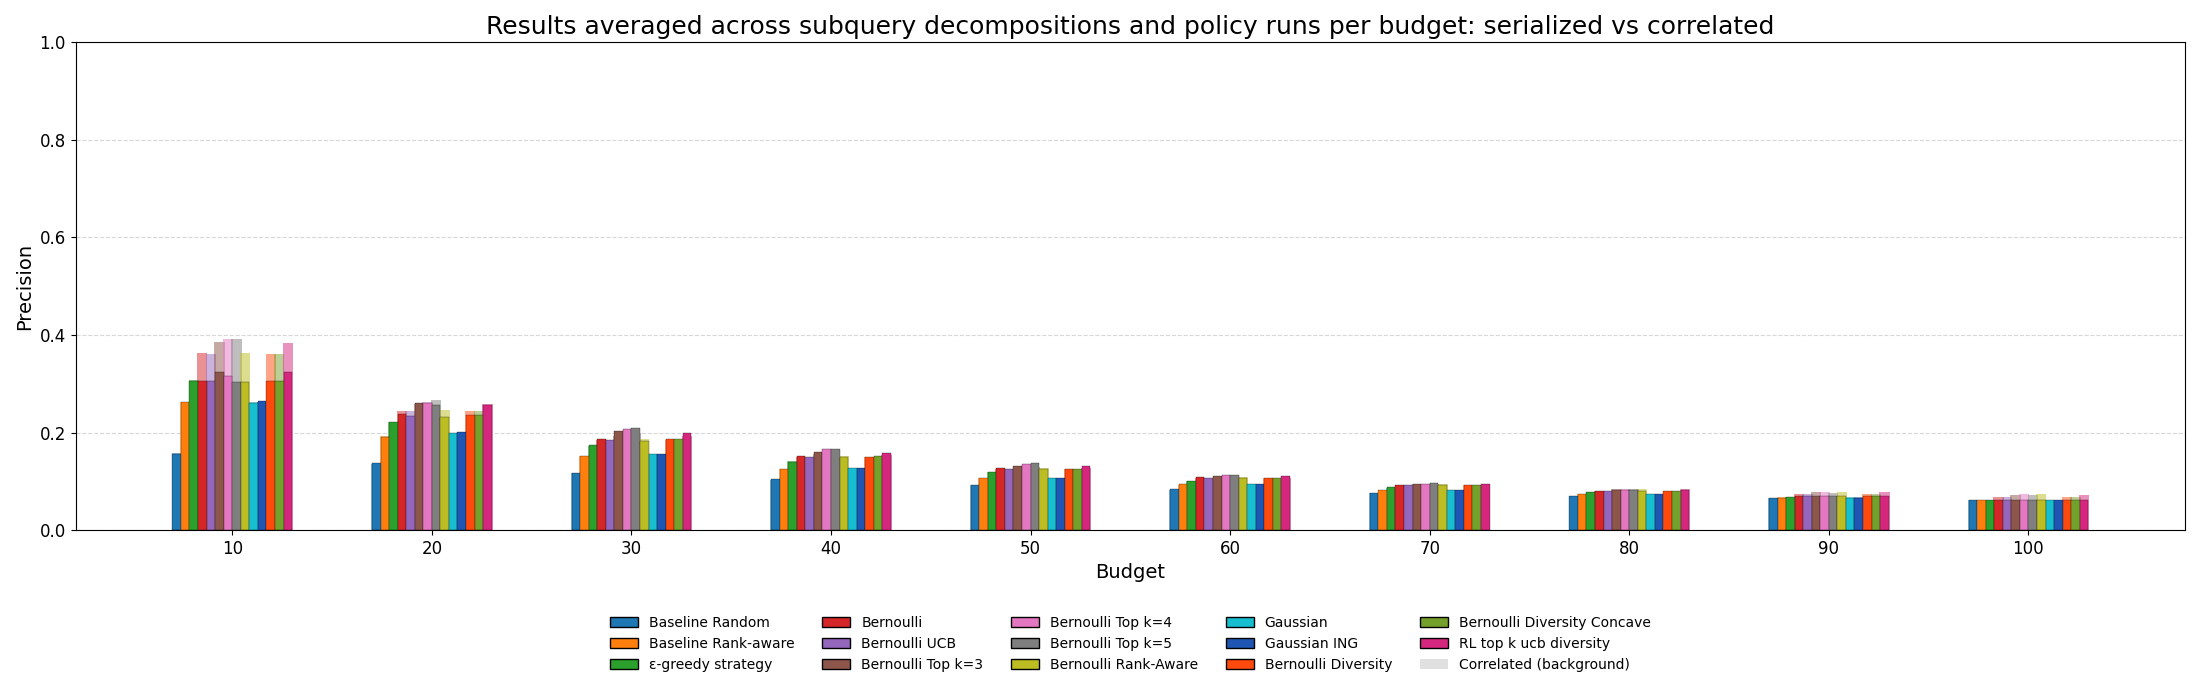
\includegraphics[width=\linewidth]{images/precision_overlay_compute_precision.png}
    \caption{Precision applying baselines and reward policies for query selection for different budgets over observed documents on the ResearchyQuestions dataset: serial vs correlated.}
    \label{fig:researchy_correlated}
\end{figure*}


